\documentclass[11pt,letterpaper]{article}
\usepackage[lmargin=1in,rmargin=1in,tmargin=1in,bmargin=1in]{geometry}
\usepackage{../style/homework}
\setbool{quotetype}{true} % True: Side; False: Under
\setbool{hideans}{false} % Student: True; Instructor: False

\usepackage{subfig}		% Subfigure Labeling
\newcommand{\usol}[2]{\underline{\hspace{#1}{\itshape #2}\hspace{#1}}}

% -------------------
% Content
% -------------------
\begin{document}

\homework{16: Due 04/10}{I should let you know, I read a book on Jiu-Jitsu, and I am prepared to throw it at you.}{Sheldon Cooper, Young Sheldon}

% Problem 1
\problem{10} For a general model, what is the difference between interpolation and extrapolation? For a linear regression, what is $R^2$ and what does it tell you? \pspace

\sol Interpolation is using a model for values between the most extreme values used to create the model. Extrapolation is using this model for values beyond the most extreme values used to create the model. \pspace

For a linear regression, $R^2$ is the coefficient of determination. This is the square of the (Pearson) regression coefficient, $R$. The coefficient of determination gives the `percentage linearity.' That is, it tells one the amount of variation in the data explained by the linear model. We only have $R^2= 1$ if the data is perfectly linear. 



\newpage



% Problem 2
\problem{10} A researcher is trying to determine if one can predict college success from a student's ACT scores. Specifically, whether one can predict a student's first semester college GPA using their ACT score. The researcher gathers data and creates a linear regression to fit the data. The researchers finds $G= 0.061A + 2.03$, where $A$ is the student's ACT scores and $G$ is the student's GPA. The researcher finds an $R^2$ value of 0.0726. 
	\begin{enumerate}[(a)]
	\item Identify $b_0$ and $b_1$ for this model.
	\item Predict a student's first semester GPA that receives an ACT score of 20. 
	\item If a student that received an ACT score of 20 had a first semester GPA of 3.010, compute the residual for this student. 
	\item Does there appear to be a (linear) relationship between ACT score and GPA? Explain using the coefficient of determination. 
	\end{enumerate} \pspace

\sol 
\begin{enumerate}[(a)]
\item We know that a simple linear regression will take the form $\widehat{y}= b_0 + b_1 x$. But given the model $G= 0.061A + 2.03$, we see that $b_0= 2.03$ and $b_1= 0.061$. \pspace

\item We have\dots
	\[
	G(20)= 0.061(20) + 2.03= 1.22 + 2.03= 3.250
	\] \pspace

\item The residual would be\dots
	\[
	e_i= \text{Actual} - \text{Predicted}= 3.010 - 3.250= -0.240
	\] \pspace

\item The $R^2$ value is $0.0726$. That is, the data is only 7.26\% linear, i.e. only 7.26\% of the variation in the data is explained by the linear model. This is a extremely low $R^2$ value. Therefore, this linear regression is a bad model. Equivalently, one's ACT score is likely a poor (linear) predictor of one's first semester college GPA. 
\end{enumerate}



\newpage



% Problem 4
\problem{10} Match each regression coefficient to its corresponding graph. 
	\begin{figure}[!ht]
	\centering
	\begin{minipage}{0.45\textwidth}
	   \centering
	   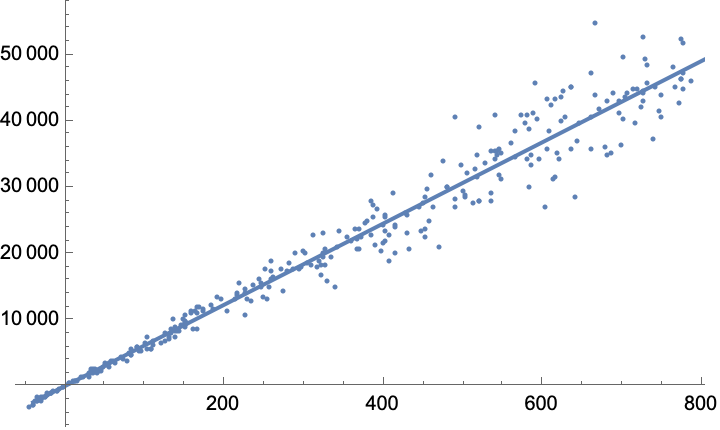
\includegraphics[width=0.9\textwidth]{reg4.png}
	   \caption*{(a)}
	\end{minipage}\hfill
	\begin{minipage}{0.45\textwidth}
	   \centering
	   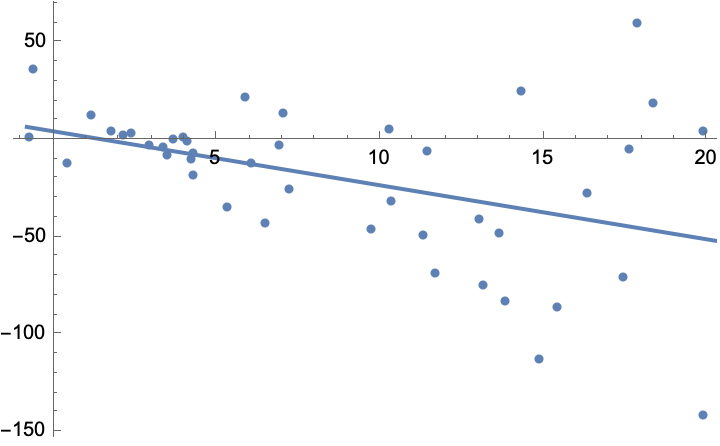
\includegraphics[width=0.9\textwidth]{reg1.png}
	   \caption*{(b)}
	\end{minipage}
	\begin{minipage}{0.45\textwidth}
	   \centering
	   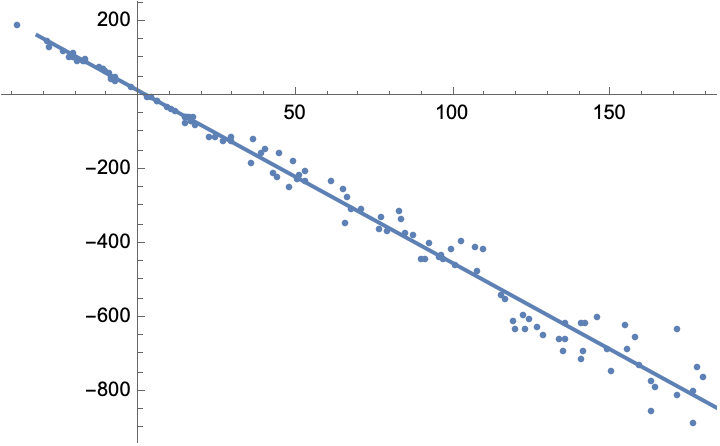
\includegraphics[width=0.9\textwidth]{reg2.png}
	   \caption*{(c)}
	\end{minipage} \hfill
	\begin{minipage}{0.45\textwidth}
	   \centering
	   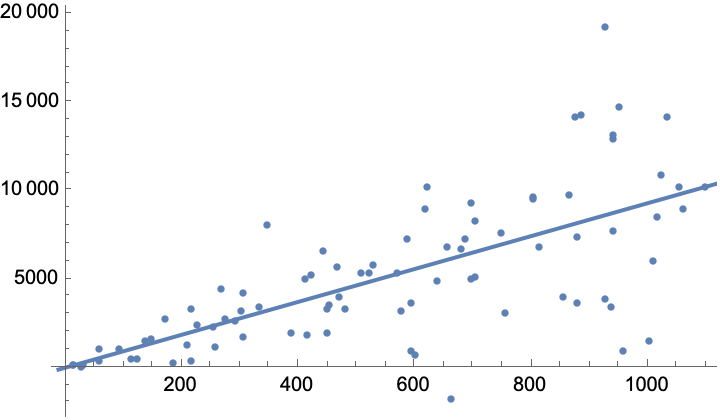
\includegraphics[width=0.9\textwidth]{reg3.png}
	   \caption*{(d)}
	\end{minipage}
	\end{figure}

\begin{enumerate}[(i)]
\item \usol{0.5cm}{a}: $R= 0.981608$
\item \usol{0.5cm}{d}: $R= 0.693245$
\item \usol{0.5cm}{b}: $R= -0.425885$
\item\usol{0.5cm}{c}: $R= -0.991438$
\end{enumerate} 


\end{document}